\chapter[Plano de Medição de TD ]{Plano de Medição de TD }

Esta sessão trará tópicos relativos ao Planejamento e Definição do GQM que será
proposto para este trabalho de medição de Débito Técnico.

\section{Planejamento do GQM}
\subsection{Estabelecer Equipe do GQM}
A equipe do GQM do Projeto de Medições para Débito Técnico (PMDT) é composta por
cinco integrantes cursandos da Disciplina de Medição e Análise de 2015-2. Estes
foram divididos em papeis dentro do grupo para a divisão de atividades de acordo
com o interesse individual. Tivemos a seguinte divisão de acordo com os respectivos
papeis:
\\


\begin{table}[ht]
\caption{Divisão dos Papeis na Equipe GQM}
\centering
\begin{tabular}{|l*{1}{c}r|}
\hline
Aluno              & Matrícula & Papel \\
\hline
Iago Golçalves & 13/0010219 &   Embasamento Teórico   \\
\hline
Lucas Mattiolli & 13/0060364 &   Embasamento Teórico \\
\hline
Tiago Assunção & 13/0051187 &   Definição do GQM  \\
\hline
Wesley Araújo & 13/00392017 &   Planejamento do GQM \\
\hline
\end{tabular}
\label{table:papeisgqm}
\end{table}

Como visto, possuímos quatro papeis para a equipe de GQM do PMDT que são fundamentais
para formar o plano de medição de Débito Técnico. Eles possuem as respectivas
responsabilidades, como podemos ver a seguir:

\begin{itemize}
  \item Embasamento Teórico, papel responsável por assegurar o grupo sobre as decisões
  práticas com solidez acadêmica adiquirida através de anos de pesquisa por pesquisadores,
  alunos, mestre e doutores.

  \item Planejamento do GQM, papel responsável por desenhar e planejar o GQM, estimar
  as equipes, projeto de atuação, área de melhoria, treinar e promover a medição
  no ambiente operacional.

  \item Definição do GQM, papel responsável por concretizar o GQM, definindo os
  Objetivos de Medição, Questões de Medição e, por fim, as métricas. Após toda a
  definição, essa equipe é responsável por validar as métricas propostas de acordo
  com o projeto.

\end{itemize}

%Area wesley
\subsection{Selecionar Área de Melhoria}
\begin{itemize}
  \item Problema: O processo de Débito Técnico proposto por  \cite{td} não possui
  um método de medição automatizado, gerando um tempo maior e, consequentemente, aumento de custo
  para para que essas medições sejam feitas de forma satisfatória.

  \item Processo: \cite{td} propõem um processo de análise do impacto de Débito Técnico,
  bem como seu custo, baseado na necessidade do mercado e em processos ja utilizados academicamente como,
  por exemplo, a estratégia SQALE (\textit{Software Quality Assessment based on Lifecycle Expectations}) e o
  Letouzey que utiliza um Modelo de Qualidade e um Modelo de Análise.
\end{itemize}

\subsection{Criar Plano de Projeto de Medição}
\begin{itemize}
  \item Cronograma: O cronograma para a execução da medição segue uma ordem cronológica
  para se conseguir resultados satisfatórios baseados em GQM. A tabela abaixo demonstra
  o cronograma:

  \begin{table}[ht]
  \caption{Divisão dos Papeis na Equipe GQM}
  \centering
  \begin{tabular}{|l*{1}{c}r|}
  \hline
  Responsavel              & Data & Papel GQM \\
  \hline
  Iago Golçalves & 19/11/2015 &   Embasamento Teórico   \\
  \hline
  Lucas Mattiolli & 19/11/2015 &   Embasamento Teórico \\
  \hline
  Tiago Assunção & 19/11/2015 &   Definição do GQM  \\
  \hline
  Wesley Araujo & 19/11/2015 &   Planejamento do GQM \\
  \hline
  \end{tabular}
  \label{table:papeisgqm}
  \end{table}

\item Organização: \cite{td} propõem um processo de análise do impacto de débito técnico,
bem como seu custo, baseado na necessidade do mercado e em processos já utilizados academicamente.
\end{itemize}

\subsection{Treinar e Promover}
\begin{itemize}
\item Objetivos de melhoria: Agilizar a medição de débito técnico no desenvolvimento de \textit{software} de forma
automatizada, baseado no trabalho de \cite{td}, sem perder a precisão das medições geradas manualmente.

\item Benefícios esperados: \cite{td} Redução do tempo para medir fatores de débito técnico, bem como a
redução de custo.

\item Impacto da medição \cite{td} Dizer mais precisamente e mais rapidamente sobre os impactos dos débitos
técnicos medidos em determinado projeto, fazendo com que o tempo seja reduzido e a visão do débito técnico, sendo
crítico ou não e seus custos, seja analisada com um ritmo equilibrado ao desenvolvimento de \textit{software}, para que não acarrete
custos ainda maiores nas análises e no desenvolvimento.

\end{itemize}
\subsection{Selecionar Projetos de Aplicação}
Para a aplicacão, os \textit{softwares} SisCot, sistema de cotações para compra de fornecedores e Aondê, \textit{software}
de acompanhamento dos gastos do governo brasileiro estão selecionados para que ocorra a medição
de débito técnico automatizado baseados no processo de \cite{td}.









%%%%%%%%%%%%%%%%%%%%%%%%%%%%%%%%%%%%%%%%%%%%%%%%%%%%%%%%%%%%%%%%%%%%%%%%%%%%%%
\section{Definição do GQM}
Este tópico traz as características definidas do nosso plano de medição, bem como
os objetivos desta, as questões aliadas aos objetivos e as suas respectivas métricas.
\subsection{Objetivos de Medição}
O objetivo de medição deste plano tem como fim possibilitar a quantificação de
Débito Técnico em um projeto de desenvolvimento de \textit{software}. O objetivo é o
seguinte:

\begin{itemize}
  \item Conhecer o quanto de Débito Técnico uma aplicação advinda de Terceiro
  possui no momento da entrega.
\end{itemize}

Para elevar o nível de detalhamento exigido para um objetivo de medição, foi
utilizado um template onde são destacados pontos sobre o objetivo, dentre eles:

\begin{itemize}
  \item Objetivo a ser analisado;
  \item Propósito;
  \item A quem diz respeito;
  \item Sob o ponto de vista de alguma determinada pessoa ou instituição;
  \item No contexto de algum ambiente em que a medição estará inserida
\end{itemize}

Dessa forma, o \textit{template} utilizado para ilustrar o objetivo de medição pode ser
visualizado na tabela \ref{table:templateobjetivo} a seguir.
\\

\begin{table}[ht]
\caption{Divisão dos Papeis na Equipe GQM}
\centering
\begin{tabular}{|l|p{7cm}|}
\hline
Analisar & Conhecer o quanto de Débito Técnico uma aplicação advinda de Terceiro
possui no momento da entrega \\
\hline
Com o propósito de & Automatizar e padronizar o processo de medição de Débito
Técnico de um \textit{Software} adquirido de terceiro \\
\hline
Com respeito a & Qualidade no Momento da Medição \\
\hline
Sob o ponto de vista de & Institução que compra um \textit{software} de um terceiro  \\
\hline
No contexto de & Projetos de Desenvolvimento de \textit{Software} adquiridos de terceiros \\
\hline
\end{tabular}
\label{table:templateobjetivo}
\end{table}

\subsection{Conduzir Entrevistas GQM}
Para alinhar o plano de medição, foi construída uma \textit{Abstraction Sheet} em conjunto
com a equipe de medição e os cliente do projeto, que são os autores de \cite{td}.
A \textit{Abstraction Sheet} leva em consideração alguns critérios que foram analisados:

\begin{itemize}
  \item Foco na Qualidade;
  \item Fatores de Variação;
  \item Hipóteses de \textit{Baseline};
  \item Impactos nas Hipóteses de \textit{Baseline}.
\end{itemize}

Em conjunto com a equipe de projeto, foi desenvolvida a seguinte tabela
\ref{table:abstraction}, ressaltando
os itens acima.
\\

\begin{table}[ht]
\caption{\textit{Abstraction Sheet}}
\centering
\begin{tabular}{p{5cm}|p{5cm}}
  \textbf{Foco de Qualidade}   & \textbf{Fatores de Variação}  \\
  Acoplamentos Aferentes, Acoplamentos Eferentes,
  Árvore de Profundidade de Herança, Falta de Coesão em Métodos, Número de filhos,
  Complexidade Ciclomática, Duplicação de Código, Documentação do Código,
  Métodos por classe
  &
  Baixa atenção dos programadores,
  ambiente não propício para desenvolvimento, pressão da alta gerência para
  a entrega da funcionalidade, optar pela falta de qualidade
  \\
\hline
\textbf{Hipóteses de \textit{Baseline}} & \textbf{Impactos nas hipóteses de \textit{Baseline}} \\

Valores baixos para acomplamento e valores altos para coesão. Baixas medidas com
Complexidade Ciclomática e Duplicação de código
&
Com o time de desenvolvimento sendo pressionado pela alta direção, é natural
que a qualidade do código seja deixada de lado para entregar a funcionalidade
no prazo adequado
\\

\end{tabular}
\label{table:abstraction}
\end{table}

\subsection{Definir Questões}
Aliadas ao objetivo de medição, tem-se questões de medição que quando respondidas
possibilitam o êxito de um objetivo. O estudo feito por \cite{oliveira} mostra que
um conjunto determinado de tipo de métricas está diretamente aliado à quantidade
de Débito Técnico de um projeto de \textit{software}. Este estudo cita o seguinte conjunto de
características de métricas:

\begin{enumerate}
  \item Métricas de Acoplamento;
  \item Métricas Relativas à Orientação a Objetos;
  \item Métricas de Estilização de Código.
\end{enumerate}

Com base no trabalho de \cite{siebra} foram elaboradas as questões de medição
para este projeto a fim de responder o objetivo citado anteriormente.

\begin{itemize}
  \item Qual o nível de acoplamento de um módulo de \textit{software}?
  \item O quão coeso está o código de um projeto?
  \item Qual a duplicidade de código?
  \item Quanto um código está documentado?
\end{itemize}

\subsection{Definir Métricas}
A fim de responder cada questão de pesquisa, são utilizadas métricas, que neste
estudo de caso foram baseadas em \cite{siebra}. Assim, as seguintes métricas
foram escolhidas:

\begin{itemize}
  \item Acoplamento Aferente
  \item Acoplamento Eferente
  \item Árvore de Profundidade de Herança
  \item Média da Falta de Coesão em Métodos
  \item Duplicação de Código
  \item Documentação do Código
  \item Métodos por classe
  \item Acoplamento entre métodos
\end{itemize}

A rastreabilidade da hierarquia do GQM com o relação de dependência entre as questões
e métricas pode ser observada na figura \ref{fig:arvore} a seguir.

\begin{figure}[h]
  \centering
  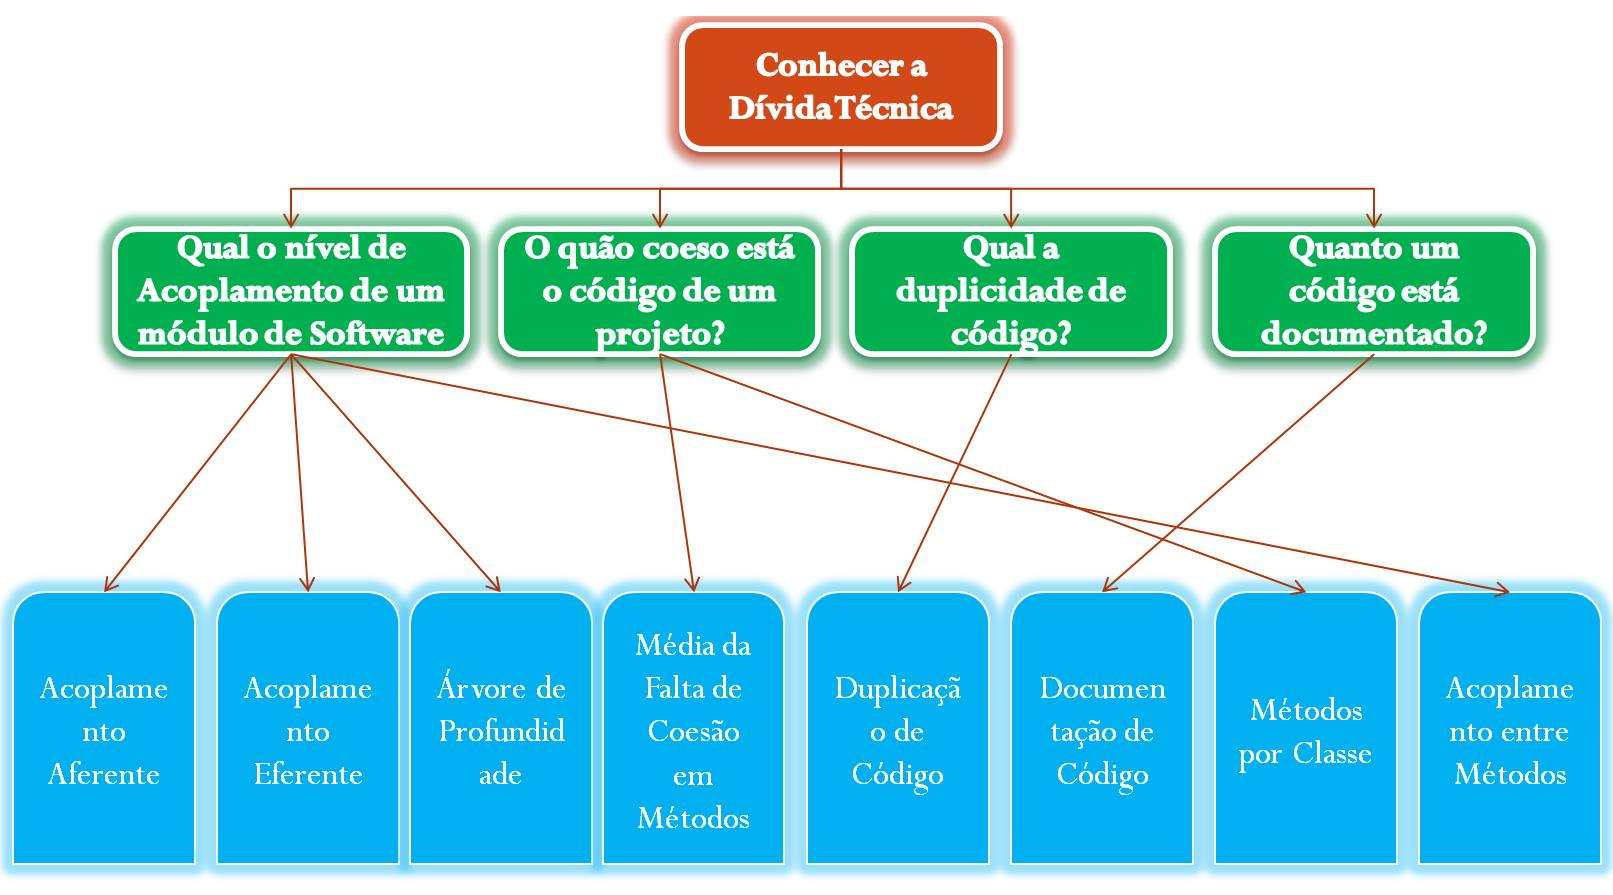
\includegraphics[width=400px, scale=1]{figuras/arvore}
  \caption{Relação entre oo objetivo de Medição, questões e métricas}
  \label{fig:arvore}
\end{figure}
